\section{Licenses}
\label{sec:ui_configure_licenses}


This dialog allows management of licenses, as stored in the configuration. \\

\begin{figure}[H]
\hspace*{-1cm}
    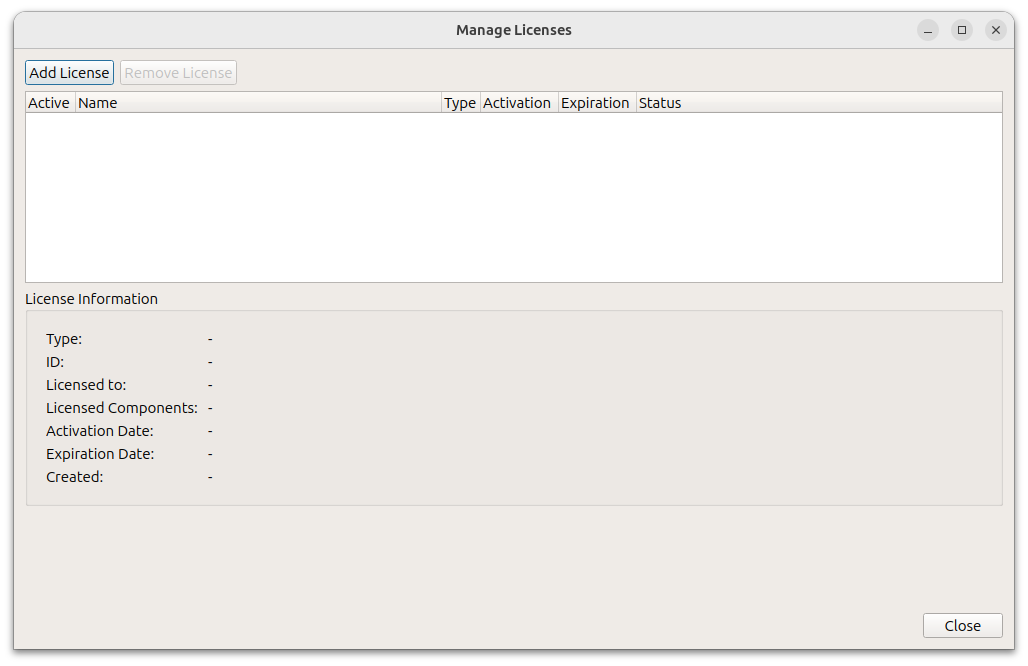
\includegraphics[width=17cm]{figures/configure_licenses.png}
  \caption{Configure Licenses}
\end{figure}

The existing licenses are used for activation / deactivation of the advanced reference reconstructor Probabilistic + IMM Reconstructor (ProbImmReconstructor) component, and to brand the application to the licensee. 
\ \\

The following elements exist:

\begin{itemize}
\item Add License button: Add a license key 
\item Remove License: Remove a selected license key
\item License list: All stored licenses, click to select
\item License information: Information for the selected license
\end{itemize}

\paragraph {License Table Content}

\begin{itemize}
\item Active: Indication if the license is the currently active license
\begin{itemize}
\item The active license is always the newest valid and most high-grade license
\item The active license will be shown in window decorations, as well as the evaluation report
\item \textbf{Note}: COMPASS supports running multiple valid licenses at the same time, but only one license will be chosen as the active license
\end{itemize}
\item Name: Unique license ID
\item Type:
\begin{itemize}
\item Free: No special license exists
\item Trial: Trial license, for limited-time testing purposes
\item Pro: Professional license given in commercial contract, commonly 1-year
\end{itemize}
\item Activation: Activation period begin date
\item Expiration: Activation period end date
\item Status: Unreadable, Invalid, Not Activated, Expired, Valid
\end{itemize}
\ \\

\paragraph {Add A License}

Click the 'Add License' button to open the following dialog:

\begin{figure}[H]
    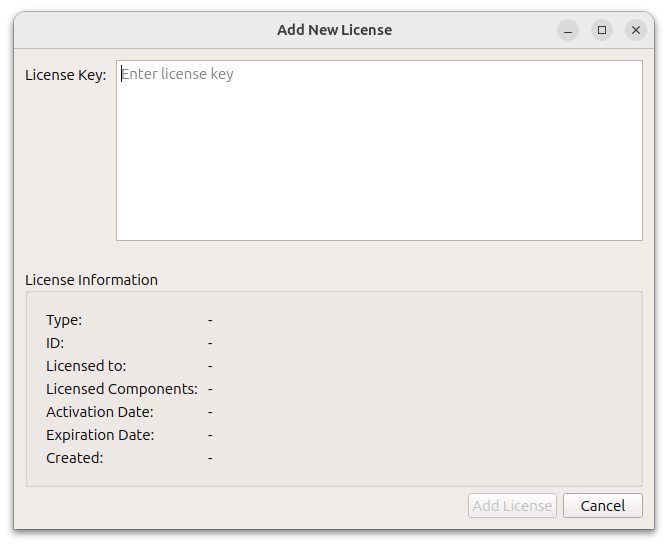
\includegraphics[width=14cm]{figures/configure_license_add.png}
  \caption{Add A License Dialog}
\end{figure}

A given license key can then be added into the text field:

\begin{figure}[H]
    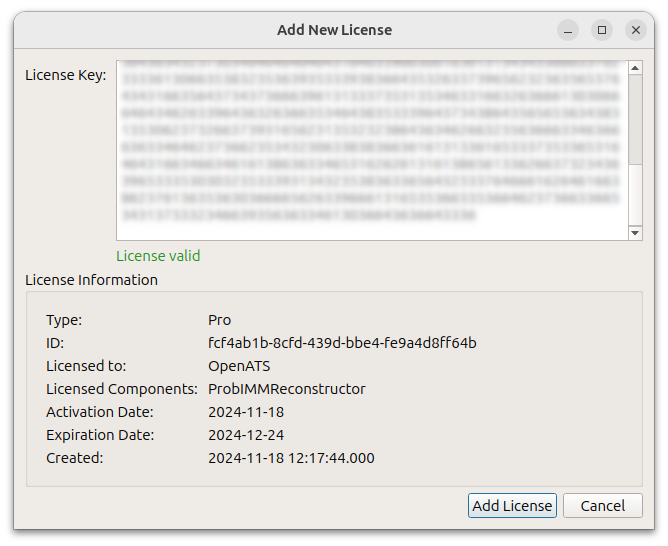
\includegraphics[width=14cm]{figures/configure_license_add2.png}
  \caption{Add A License Key}
\end{figure}

To add the license, use the 'Add License' button. 
\textbf{Note} that invalid or expired licenses cannot be added.

\begin{figure}[H]
    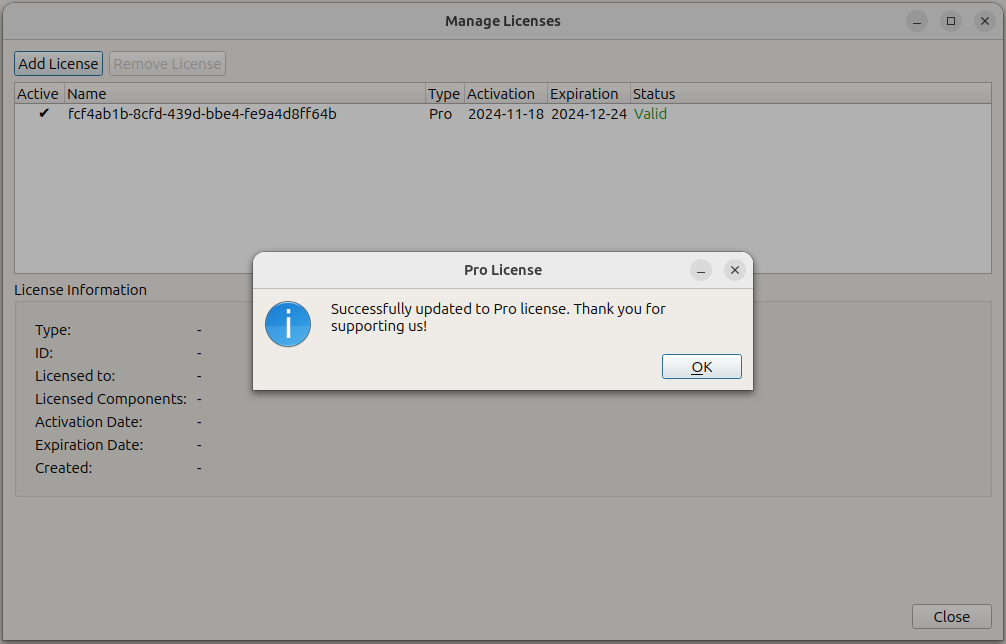
\includegraphics[width=14cm]{figures/configure_license_add3.png}
  \caption{Added A License Key}
\end{figure}

If any of the existing licenses is valid (readable, verifiable and the current date falls inside the activation period), the components contained in the license will be available. \\

If interest exists, (free, time-limited) trial licenses can be obtained by contacting \href{mailto:compass@openats.at}{compass@openats.at}.
